\subsection{Retour d'expérience sur le Xeon Phi}
Le Xeon Phi est un co-processeur conçut par Intel.
%
Il s'agît d'une carte branchée en PCI express et qui permet de faire du calcul déporté.
%
Ce co-processeur est composé de 60 coeurs de calcul généralistes.
%
Ces coeurs de calcul supportent le jeu d'instructions x86 et ont la particularité de pouvoir maintenir 4 contextes d'exécution simultanément.
%
Il s'agit de la technologie HyperThreading ou SMT\footnote{Simultaneous Multi Threading}.
%
Un changement de contexte est effectuer à chaque cycle.
%
L'utilisation de plusieurs threads par coeur à l'avantage de pouvoir masquer les temps d'attentes mémoire.
%
En parlant de mémoire, celle du Xeon Phi est en anneau et utilise l'interconnect (Fig.~\ref{fig:interconnect}).

%   (-_-)   %
\begin{figure}[t!]
  \centering
  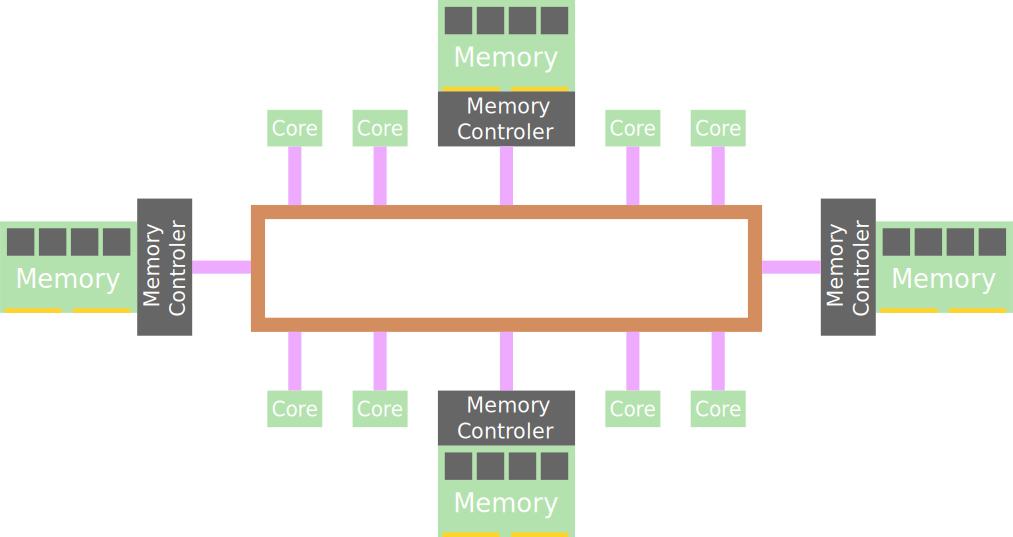
\includegraphics[width=\textwidth]{interconnect}
  \caption{Architecture en anneau du Xeon Phi.}
  \label{fig:interconnect}
\end{figure}


Cette mémoire nous fournit de très bon débit mémoire comparé à la mémoire de la carte mère hôte.
%
Pour cette raison, il peut être intéressant de tester nos noyaux d'algèbre linéaire creuse sur cet accélérateur.
%
L'accélération maximale est de 120 par rapport à un coeur du Xeon Phi (Fig.~\ref{fig:res_spmv_xeon_phi}).
%
Mais il faut rappeler que ces coeurs ne sont pas faits pour exécuter du code séquentiel.
%
Les instructions sont exécutées dans l'ordre (in-order) et il n'y a donc pas de parallélisme d'instructions.
%
De plus, la fréquence d'horloge est basse (1,2~GHz) et le thread est exécuté un cycle sur 2 (600~MHz).
%
Il est donc très simple d'obtenir une bonne accélération par rapport à un coeur du Xeon Phi.

%   (-_-)   %
\begin{figure}[t!]
  \centering
  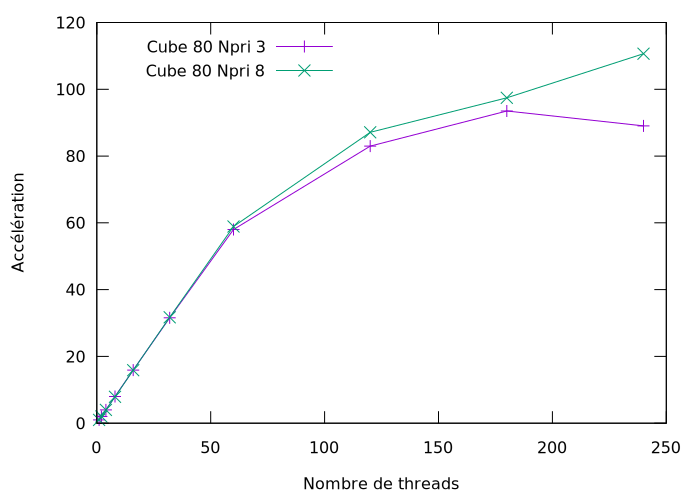
\includegraphics[width=0.7\textwidth]{res_spmv_xeon_phi}
  \caption{Résultat sur produit matrice vecteur creux sur Xeon Phi.}
  \label{fig:res_spmv_xeon_phi}
\end{figure}



Par contre, si nous comparons le temps qu'il a fallu au Xeon Phi pour faire la multiplication par rapport au temps que met les deux processeurs hôtes à faire la même opération, le Xeon Phi ne met que 2 fois moins de temps (0,110~s sur 2 processeurs Xeon contre 0.058~s pour le Xeon Phi avec 8 variables primaires).
%
Ce qui est déjà bien mais ces résultats ne sont pas suffisant pour utiliser des Xeon Phi.
%
Pour comprendre pourquoi, il faut regarder le fonctionnement du Xeon Phi.
%
En effet, il y a deux modes de programmation du Xeon Phi :
\begin{itemize}
    \item le mode natif, qui consiste à faire tourner un noyau Linux sur le Xeon Phi et à l'utiliser comme un noeud de calcul;
    \item le mode déporté, qui consiste à l'utiliser comme un accélérateur, à la manière d'un GPU.
\end{itemize}

Dans le mode natif, le code du simulateur de réservoir doit aussi tourner sur le Xeon Phi.
%
Or les parties séquentielles du code s'exécutent environ 10 fois moins vite que sur un processeur classique.
%
Donc les accélérations que nous obtenons sur les noyaux de calcul parallèle seront perdues à cause des parties séquentielle du code.


Quant au mode déporté, pour pouvoir exécuter les noyaux de calcul sur le Xeon Phi, nous devons transférer les données qui seront utilisées et/ou produites.
%
Dans le cas du produit matrice vecteur creux, nous devons d'abord transférer la matrice et le vecteur, puis à la fin du calcul nous devons récupérer un vecteur.
%
Or, ces transferts coûtent du temps et ce temps cumulé à l'exécution du noyau de calcul est plus long que l'exécution du code sur les processeurs hôtes.
%
De plus, ce mode ajoute de la complexité au code qui doit maintenant avoir un support des transferts mémoires.
%
Cette complexité peut bien entendu être masqué par un runtime à base de tâches qui s'occupera des transferts mémoire à notre place.
%
Mais le travail nécessaire reste trop important par rapport aux gains obtenus.
